\chapter{Human Tissue}

\section{Introduction}


\section{Methods}

\subsection{Potting}

The geometry of human lumbar vertebrae varies considerably to that of the bovine
tail vertebrae from which this methodology is based. This is characterised by
much larger posterior elements with the facets extending much lower, below the
bottom of the vertebral body. Hence, to correctly pot the human vertebrae much
more cement must be used, especially for the posterior end-cap, in order to
cover the bottom of the vertebral body and the extending posterior elements.
This means that much more of the posterior elements are constrained, therefore
restricting the rotation of the vertebral body endplates under axial load. In
addition to this the larger posterior elements which are captured within the
PMMA end-caps will transmit load and take a greater share of the load when
compared to the bovine tail vertebrae. Given that vertebroplasty attempts to
restore the stiffness of the vertebral body and that there is no understanding
of specifically how the loads are shared between the vertebral body and
posterior element, this presents a problem.

A solution to this is to remove the posterior elements, following such methods
as \cite{Wijayathunga2008,RobsonBrown2014}, where only the vertebral body is
modelled. This allows the stiffness of the vertebral body alone to be captured
and modelled. The posterior elements were removed by cutting through the
pedicles at the narrowest part, limiting damage to the region.

To pot the specimens that now lack a spinal canal, a retort stand was used to
hold the vertebra, ensuring that both endplates were level on average. The
specimen was then lowered down into the potting container leaving 5 mm between
the bottom of the vertebra and the container. PMMA was poured into the container
until the entire of the endplate was touching cement, with the edges of the
vertebral body covered. Care needed to be taken to ensure all of the endplate
was in contact with cement, given the extent of osteophytes creating non-flat
surfaces in some of the more degenerated specimens. The other side of the
vertebra was potted in a similar manner, however, due to the constraints of the
potting container a measured quantity of cement was poured prior to lowering the
vertebra into it. A spirit level ensured parallel end-caps.

\subsection{Loading}

Following previous studies \cite{Wijayathunga2008}, the vertebrae were loaded
with an initial maximum load of 800 N for similarly osteoporotic vertebrae.
However, after loading two of the initial set of vertebrae the stiffness
continued to increase up to maximum 800 N. Following loads up to 2000 N showed
that the stiffness reached a maximum between 1300 and 2000 N, with three of the
initial four specimens showing some degree of failure in the final 400 N of
loading.

\subsubsection{Maximum Stiffness Measurement}

The maximum stiffness of the vertebra was found in the same fashion as with the
bovine tail vertebrae - measuring the stiffness of segments at increments over
the length of the curve. Given that damage, especially for the intact specimens,
needs to be avoided the maximum loads used are on the conservative side. This
can mean that the maximum stiffness is potentially at the end of the data set or
that the stiffness is still increasing at the load cut off. The solution to the
latter would require a prediction of the yield point prior to experimental
loading (discussed in Section \ref{predYield}), while the former could
potentially be solved by using smaller segment sizes when measuring the
stiffness from load - displacement results.

To allow the effect of segment size (the length of each section from which the
stiffness is found) and increment size (the size of each increment defining the
start point of each segment), the maximum stiffness finding Matlab code was
rewritten in Python. This function could then be iterated over, reporting the
maximum stiffness when using an increment size of between 1 and 100 data points
(the distance between two data points corresponds to 0.0017 mm). Changing the
increment size becomes a verification of the results using an increment size of
1 data point, given that the only negative of using the smallest possible
increment size is computational cost, which is negligible here.

\begin{figure}[ht!]
  \centering
  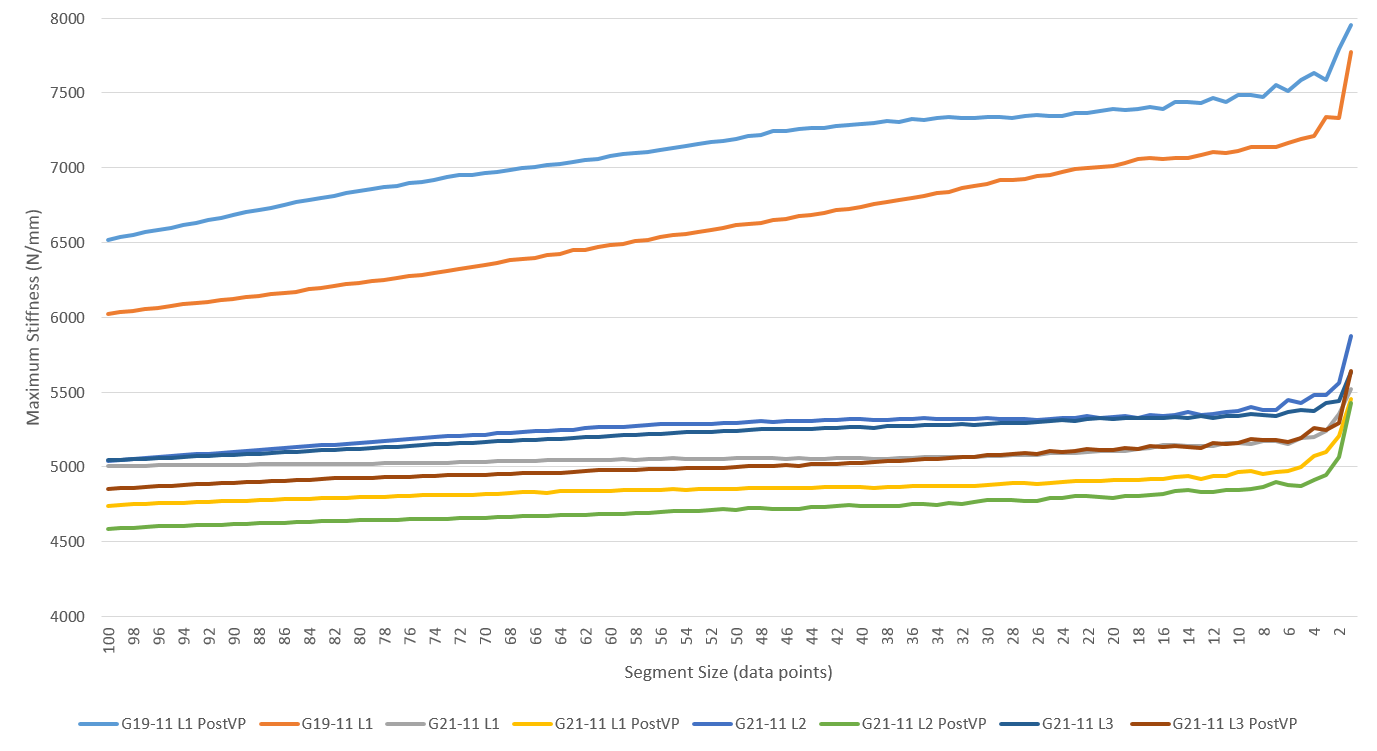
\includegraphics[width=6in]{Chapters/Chapter_HT_images/findStiffness_1incr.png}
  \caption{The effect of reducing the segment size on the maximum stiffness
    reported from four human vertebrae loaded to 2000 N pre and post
    augmentation. Using an increment size of 1 data point (0.0017 mm) and
    segment sizes of 100 to 1 data point (0.17 mm to 0.0017 mm).}
  \label{fig:findStiffness_1incr}
\end{figure}

\begin{figure}[ht!]
  \centering
  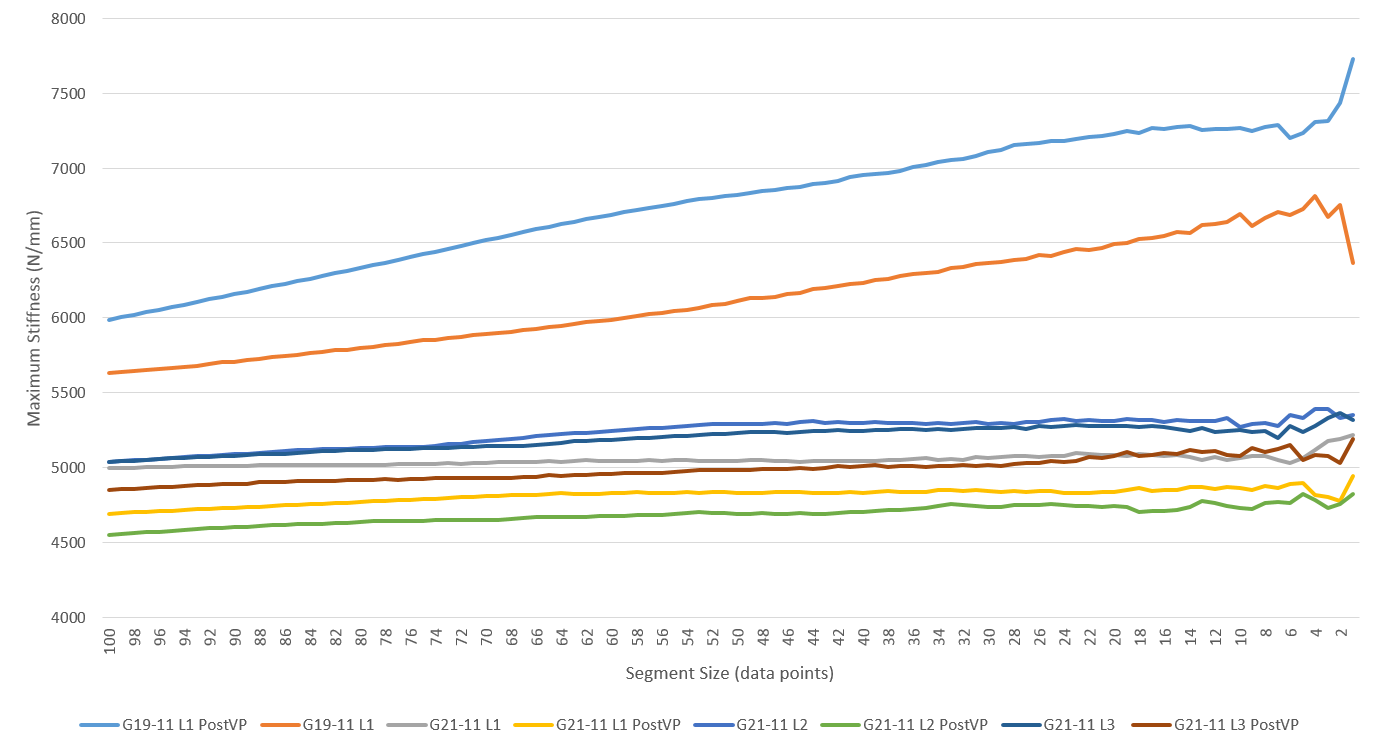
\includegraphics[width=6in]{Chapters/Chapter_HT_images/findStiffness_20incr.png}
  \caption{The effect of reducing the segment size on the maximum stiffness
    reported from four human vertebrae loaded to 2000 N pre and post
    augmentation. Using an increment size of 20 data points (0.0037 mm) and
    segment sizes of 100 to 1 data point (0.17 mm to 0.0017 mm).}
  \label{fig:findStiffness_20incr}
\end{figure}

Using an increment size of 1 data points width, as shown in Figure
\ref{fig:findStiffness_1incr} shows a smaller variation across the range of
segment sizes compared to using 20 points in Figure
\ref{fig:findStiffness_20incr}. The effect of both segment size and increment
size is especially evident for the two G19-11 L1 vertebrae both intact and post
augmentation where the stiffness continues to increase until the end of the test
at 2000 N. Meaning that there is a much smaller linear region for these two
specimens, hence requiring a smaller segment size to measure the largest
gradient.

Choosing values for the segment size to use moving forwards becomes difficult
given the large effect it can have on the measured maximum stiffness (a range of
over 1000 N/mm in the case the two G19-11 L1 tests). The segment size needs to
be small enough to capture the maximum stiffness while avoiding the noise when
using a segment size below 18 data points. Hence, a value of 20 data points was
chosen, a value that avoids the noise while being on the plateau of the lines.


\subsubsection{Repeated Loading}

Given the nature of the test, attempting to limit damage to the vertebrae,
especially during their initial intact load, the ability to derive errors
becomes difficult especially from a single load. To attempt to understand this
error four vertebrae having undergone augmentation were tested three more times
in an iterative fashion, removing each from the load testing machine, testing
the next specimen in the set and repeating. Removing the vertebrae from their
steel housing (instead of three tests while seated in the steel housing) allowed
the error in loading position and setup to be tested along with repeated loading
of the vertebrae to be tested.

The results of repeated loading can be seen in Figure \ref{fig:exp_repeats}. All
four specimens show a reduced stiffness for the repeated loads following the
initial load, for which there are a few possible reasons. One possibility for
the reduction in stiffness is that it is a consequence of the freeze thaw cycle
that occurred between these tests. The second possibility is that the vertebrae
were still partially frozen while the testing took place. Finally, it could be
due to damage being caused during the initial load to 2000 N, shown in Figures
\ref{fig:G19-11_L1} to \ref{fig:G21-11_L3} it is possible to see slight failure
in the three G21-11 vertebrae, although failure cannot be seen in the G19-11 L1
vertebrae. The frozen bar in Figure \ref{fig:exp_repeats} shows how the
stiffness increases when the vertebrae are completely frozen, potentially
helping to explain the drop in stiffness found in the repeats. Further tests
will be carried out with three more repeats following another freeze thaw cycle
to attempt to answer this.

The iterative reduction in stiffness for the G21-11 L2 vertebrae can be
explained as damage being caused after each iteration. This can be seen in
Figure \ref{fig:G21-11_L2}, with the three repeats each showing a yielding
before the 1600 N limit and a smaller maximum load and stiffness after each
repeat.

Figures \ref{fig:G19-11_L1} through \ref{fig:G21-11_L3} show the data for the
loading, from which the maximum stiffness values are found. This excludes the
initial cyclic loading, starts the loading at 50 N and displacement at 0 mm.

\begin{figure}[!h]
  \centering
  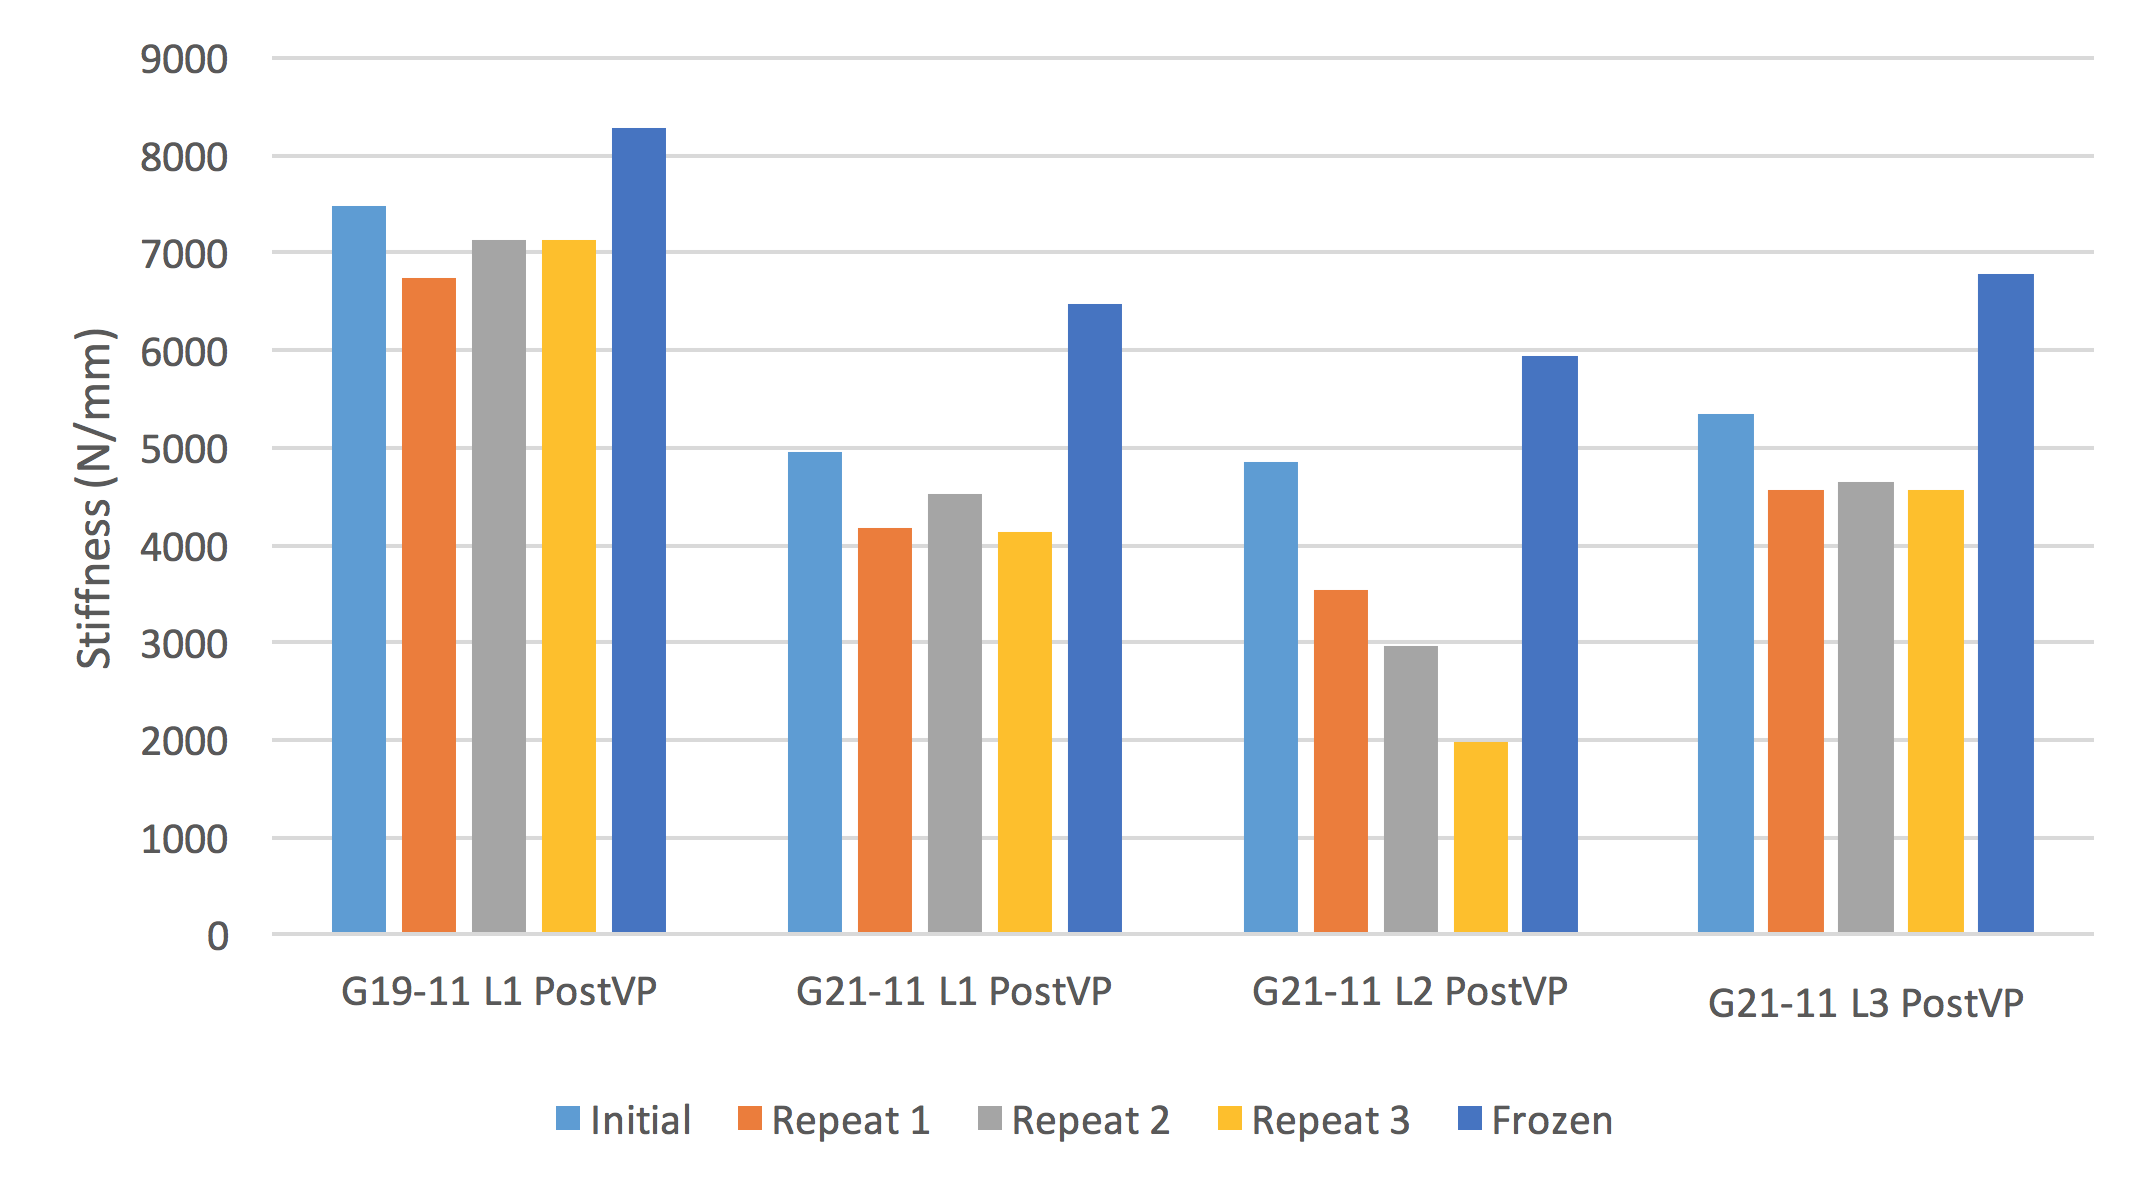
\includegraphics[width=6in]{Chapters/Chapter_HT_images/experimental_repeats.png}
  \caption{The stiffness of four augmented vertebral specimens over the course
    of an initial load, three repeated loads and a load while frozen. The intact
    specimen was loaded until 2000 N while the remaining four were loaded until
    1600 N.}
  \label{fig:exp_repeats}
\end{figure}


\begin{figure}[ht!]
  \centering
  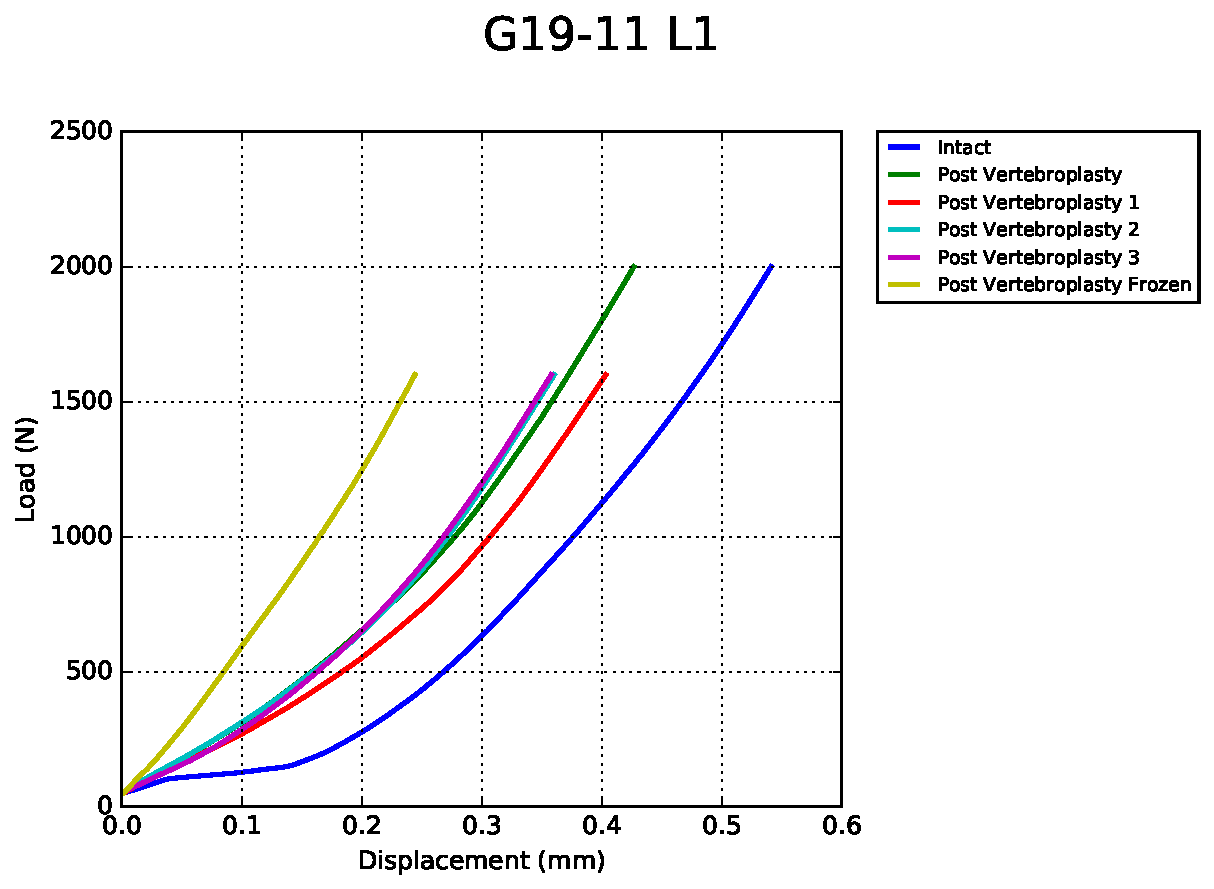
\includegraphics[width=4in]{Chapters/Chapter_HT_images/G19-11_L1.pdf}
  \caption{The load - displacement results for the G19-11 L1 vertebra. Showing
    results of the intact load and post augmentation load up to 2000 N and the
    repeats and frozen load up to 1600 N.}
  \label{fig:G19-11_L1}
\end{figure}

\begin{figure}[ht!]
  \centering
  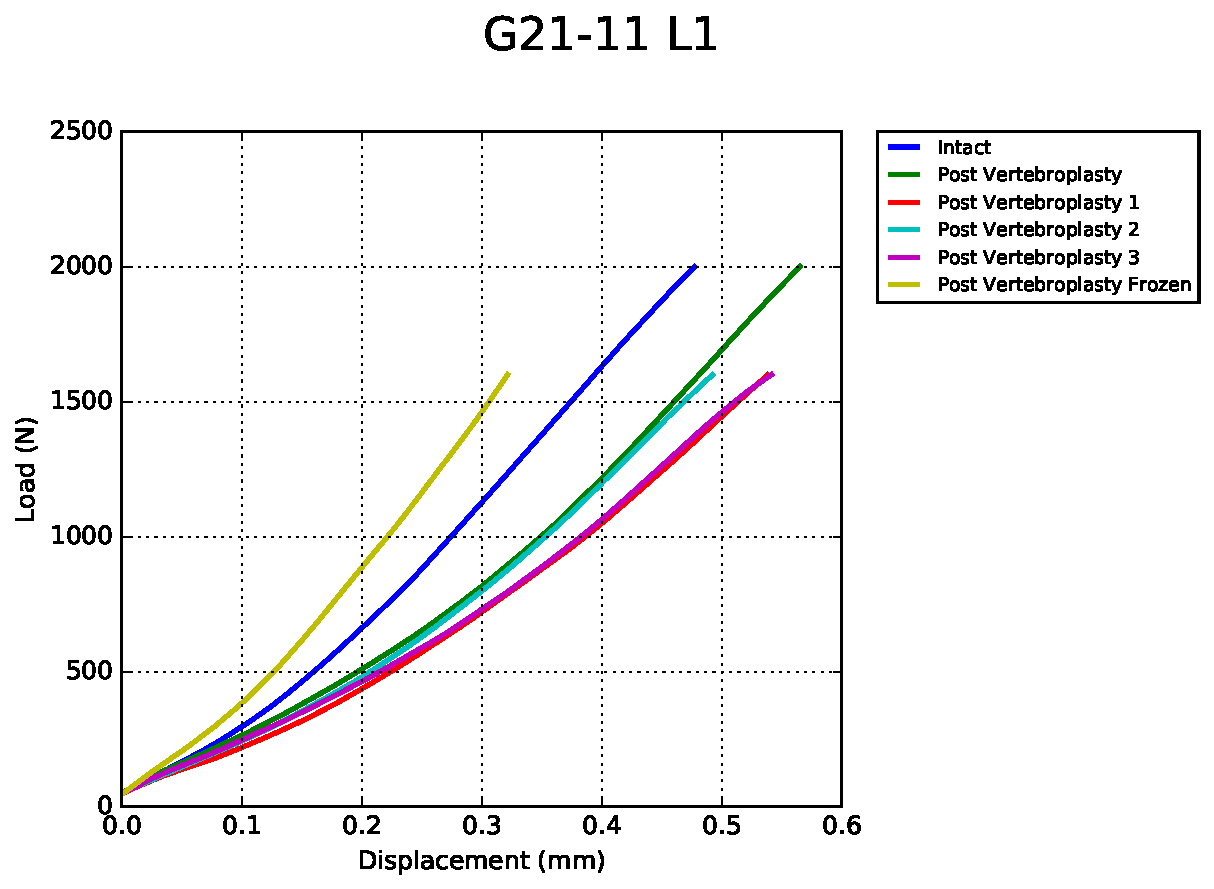
\includegraphics[width=4in]{Chapters/Chapter_HT_images/G21-11_L1.pdf}
  \caption{The load - displacement results for the G21-11 L1 vertebra. Showing
    results of the intact load and post augmentation load up to 2000 N and the
    repeats and frozen load up to 1600 N.}
  \label{fig:G21-11_L1}
\end{figure}

\begin{figure}[ht!]
  \centering
  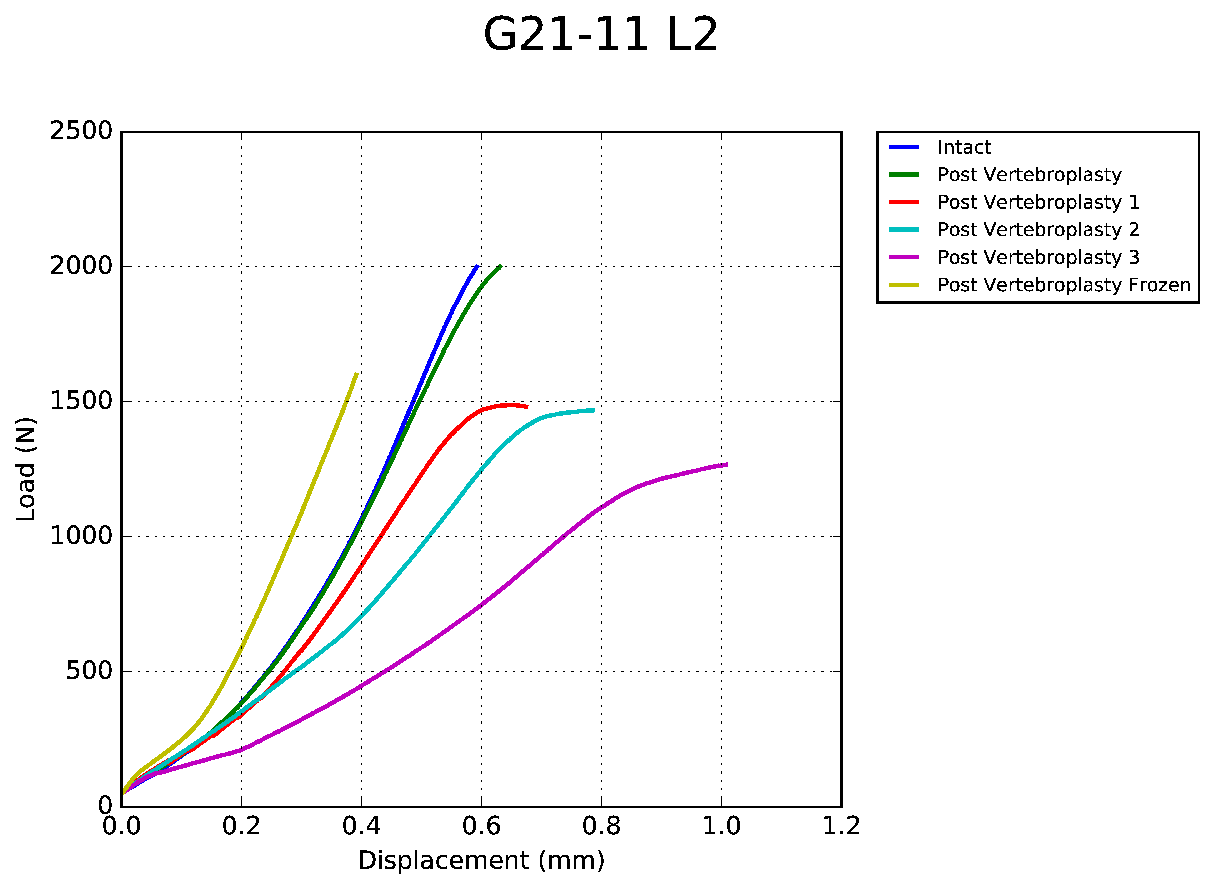
\includegraphics[width=4in]{Chapters/Chapter_HT_images/G21-11_L2.pdf}
  \caption{The load - displacement results for the G21-11 L2 vertebra. Showing
    results of the intact load and post augmentation load up to 2000 N and the
    repeats and frozen load up to 1600 N.}
  \label{fig:G21-11_L2}
\end{figure}

\begin{figure}[ht!]
  \centering
  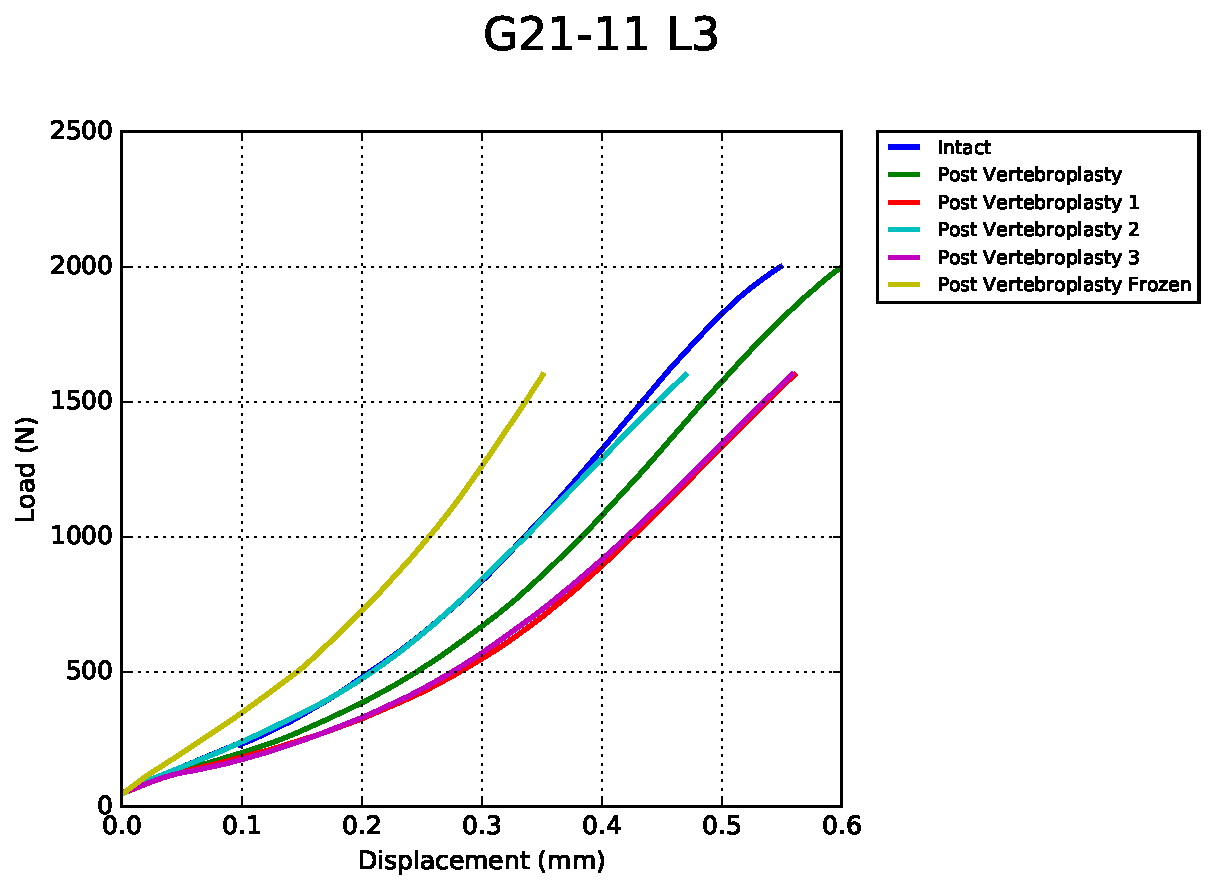
\includegraphics[width=4in]{Chapters/Chapter_HT_images/G21-11_L3.pdf}
  \caption{The load - displacement results for the G21-11 L3 vertebra. Showing
    results of the intact load and post augmentation load up to 2000 N and the
    repeats and frozen load up to 1600 N.}
  \label{fig:G21-11_L3}
\end{figure}






\subsection{Vertebroplasty}

Despite the development of methods for the augmentation of bovine tail
vertebrae, the methods for augmenting human vertebrae were altered due to the
different geometry and density. The human vertebrae, being much less dense, did
not require the vertebroplasty needle to be inserted with the aid of a mallet.
Instead the needle could be pushed by hand through the cortical shell and into
the vertebral body.

An additional difference was the approach with the needle, instead of entering
the vertebrae through their pedicles an oblique approach was adopted. This was
due to variation in pedicle diameter between the L1 - L5 lumbar levels and
therefore the potential to damage the region and its load sharing capabilities.
The oblique approach therefore avoided creating this damage to the pedicle-canal
region, especially for the vertebrae with narrower pedicles and instead created
much less damage to the vertebral body.

A final difference to the needle insertion methods was a change to the needle.
Here, a side opening needle was used, allowing the cement to be directed into
the anterior-centre region of the vertebral body as opposed to directly out of
the needle end.

An attempted 20 \% fill was used for the vertebrae, measuring the volume of the vertebral body from the $\mu$CT scans prior to augmentation.
However, despite stopping the injection upon cement leakage through vascular channels leading from the vertebral body surface inwards, cement loss occurred.
In addition to this, cement was also lost in the needle itself, where as the cement set the amount of cement remaining in the needle became difficult to measure.
This meant that the cement fill could not be measured though the amount of PMMA leaving the syringe due to leakage and needle losses.
Hence cement fill volume was measured using segmented $\mu$CT scans, the methodology of which is described below.

\subsection{Vertebrae Characteristics}

Identifying the different characteristics for the set of lumbar vertebrae has
importance in understanding trends and relationships between the experimental
and computational results. For example a larger degree of anisotropy and hence
more directionality aligned trabeculae would potentially give a more
experimentally stiff vertebra, despite otherwise similar characteristics. Given
that much of the vertebral characteristics depend on the trabecular structure it
is important to understand how this varies between specimens. Furthermore, any
calculations originating from a description of the trabecular structure require
a correct threshold to be applied to the $\mu$CT scan. This threshold describes
the limit of the trabecular bone and hence the start of either marrow or empty
space. To enable a fair comparison between vertebrae a region of interest was
selected from the vertebral body. Given the large variation in cortical shell
thickness, along with certain vertebrae containing large osteophytes and other
extra bone growth, the region of interest (ROI) was selected to be the largest
cylinder that could fit within the vertebral body while not capturing any of the
cortical shell.

\subsubsection{Histograms}

In order to understand the spread of brightness' from the set of lumbar the
histograms of the ROIs were plotted (Figure \ref{fig:normalisedhistogram}).

\begin{figure}[ht!]
  \centering
  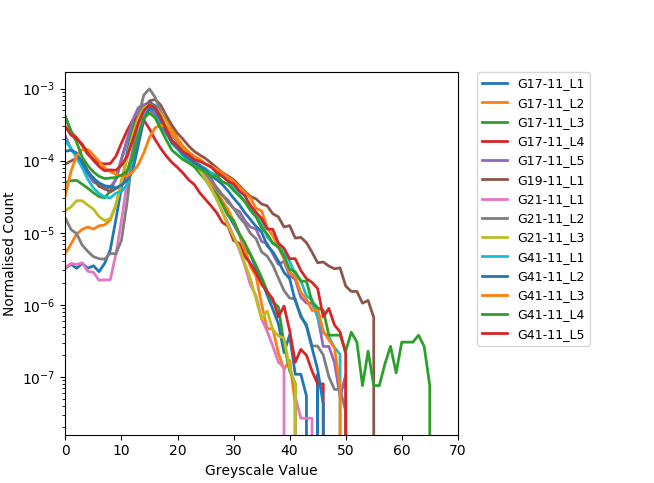
\includegraphics[width=4in]{Chapters/Chapter_HT_images/Normalised_Histogram.png}
  \caption{The normalised (with respect to the volume of the ROI) histogram data
    for the 14 lumbar vertebrae.}
  \label{fig:normalisedhistogram}
\end{figure}

The lower greyscale values represent the empty space within the ROI which
translates to regions where the bone marrow has exited the region, most likely
during the freeze thaw cycles. The peak in the histogram at an approximate
greyscale value of 16 is due to the bone marrow. The remaining portion of the
histogram represents bone, where variation is due to the differences in the
mineral content of the bone, with more mineralised bone appearing brighter on
$\mu$CT scans. The specimens ROIs that contain the brighter values are those
that contain osteophytes that contain more dense bone than the other cortical
shell, for example G19-11 L1.

\subsubsection{Threshold Optimisation}


The full resolution scan is imported into imageJ where the threshold
optimisation is carried out. The BoneJ plugin for imageJ is used for all of the
trabecular structure metrics, with the optimise threshold tool being the focus
here. This tool is run on the region of interest using the default settings for
the connectivity options seen in Table \ref{tab:bonej}. This chooses a threshold
based on the peak in a connectivity against threshold plot and reports that
value. These values can be seen in Table \ref{tab:optTH}, showing considerable
across the range of vertebrae. However, the differences in these suggested
thresholds can grouped with the spine, for example: the G17 spine has a range
between 15 to 17, while the G41 spine has an range between 18 to 20. This
promotes the idea that these differences are due to the bone mineralisation of
the bone, especially given that the G17 spine is from a Female and G41 from a
male.

However, given that the chosen value for the threshold will directly impact the
reported metrics, a consistent value was chosen of 18. Using lower or
higher values for the threshold usually results in the trabeculae being
described as thicker or thinner respectively. Hence, the difference in the
mineralisation between specimens will still be captured when using a fixed
threshold, given that the binary image will be down sampled before material
properties are acquired. The results in Table \ref{tab:bv_tv_anis} show the BV /
TV data and degree of anisotropy values for the 14 specimens using the fixed
threshold of 18. Similar trends to what could be seen from the optimise
threshold results can be seen in the BV/TV data, with grouping between the
spines evident.

\begin{table}[ht!]
	\caption{Settings used for the ImageJ plugin, BoneJ: Optimise Threshold.}
	\label{tab:bonej}
	\centering
	\begin{tabular}{c|c}
    Options & Values \\
    \hline
    \hline
    Tests & 11  \\
    Range & 0.2 \\
    Subvolume Size & 256 \\
    Erosian Cycles & 0 \\
    Dilation Cycles & 0 \\
    \hline
	\end{tabular}
\end{table}

\begin{table}[ht!]
	\caption{The suggested threshold from the optimise threshold BoneJ tool for
    the 14 lumbar vertebrae in the set.}
	\label{tab:optTH}
	\centering
	\begin{tabular}{c|c}
    Specimen    & Suggested Threshold   \\ \hline \hline
    G17-11\_L1 & 17 \\
    G17-11\_L2 & 16\\
    G17-11\_L3 & 16\\
    G17-11\_L4 & 15\\
    G17-11\_L5 & 16\\
    G19-11\_L1 & 23\\
    G21-11\_L1 & 18\\
    G21-11\_L2 & 19\\
    G21-11\_L3 & 19\\
    G41-11\_L1 & 20\\
    G41-11\_L2 & 19\\
    G41-11\_L3 & 18\\
    G41-11\_L4 & 19\\
    G41-11\_L5 & 18\\
    \hline
	\end{tabular}
\end{table}

\begin{table}[ht!]
	\caption{BV/TV and degree of anisotropy (DA) values found using the ImageJ
    plugin BoneJ tools Volume Fraction and Annisotropy respectively using a
    threshold of 18.}
	\label{tab:bv_tv_anis}
	\centering
	\begin{tabular}{c|c|c}
    Specimen                       & BV/TV & DA\\ \hline \hline
    G17-11\_L1  & 0.174 & 0.387 \\
    G17-11\_L2  & 0.17  & 0.364\\
    G17-11\_L3  & 0.137 & 0.359\\
    G17-11\_L4  & 0.127 & 0.418\\
    G17-11\_L5  & 0.187 & 0.341\\
    G19-11\_L1  & 0.391 & 0.199\\
    G21-11\_L1  & 0.255 & 0.327\\
    G21-11\_L2  & 0.267 & 0.231\\
    G21-11\_L3  & 0.281 & 0.301\\
    G41-11\_L1  & 0.257 & 0.239\\
    G41-11\_L2  & 0.241 & 0.338\\
    G41-11\_L3  & 0.244 & 0.348\\
    G41-11\_L4  & 0.247 & 0.371\\
    G41-11\_L5  & 0.249 & 0.186\\
    \hline
	\end{tabular}
\end{table}




\subsection{Modelling}

Given the aims of the project - to include the models generated here into a
larger set of vertebral models for use in statistical shape modelling, it is
useful to model the vertebrae in a scanner independent method. A method for
doing this (BV/TV modelling method) uses a full resolution scan with the bone
regions segmented using a threshold. This full resolution segmented scan is then
downsampled to voxels with edge length of 1 mm, meaning that each voxel has a
greyscale value proportional to the BV/TV value for the region captured by that
voxel. Areas that contain more bone will therefore have a higher greyscale
value. This method is purely dependant on the threshold selected defining the
bone and hence, given that threshold values can be repeatedly and correctly
selected, is scanner independent.

\subsubsection{BV/TV Modelling Method}

The method follows that found in a study by Robson Brown et al.
\cite{RobsonBrown2014} with a few minor changes. The scans are converted into a
stack of TIFF files using an in house Matlab script, which in addition reduces
the 16 bit file to 8 bit images.



The set of vertebral specimens were split at this stage into two sets, allowing
an understanding of the effect of specimen specific thresholds for the vertebral
models, these sets used a threshold of 21 for the Uniform test and their BoneJ
predicted value for the Different Threshold Set. Following the application of
the threshold (creating a binary image stack) a Gaussian filter with $
\sigma_{x,y,z} = 1 $ was applied in order to remove speckling found surrounding
the end-caps. The two stacks of images are then imported into ScanIP; carried
out by opening one stack of images (the original stack) and then importing a
second background (the binary image stack). Both backgrounds are downsampled to
voxel sizes of 1 mm$^3$, with the (originally) binary stack being used to create
the mask for the vertebrae and the original stack being used for the end-caps.
Greyscale material properties for the vertebral mask are taken from the binary
stack, while the remainder of the methods follow the same process as the
original method.

\begin{figure}[ht]
  \centering
  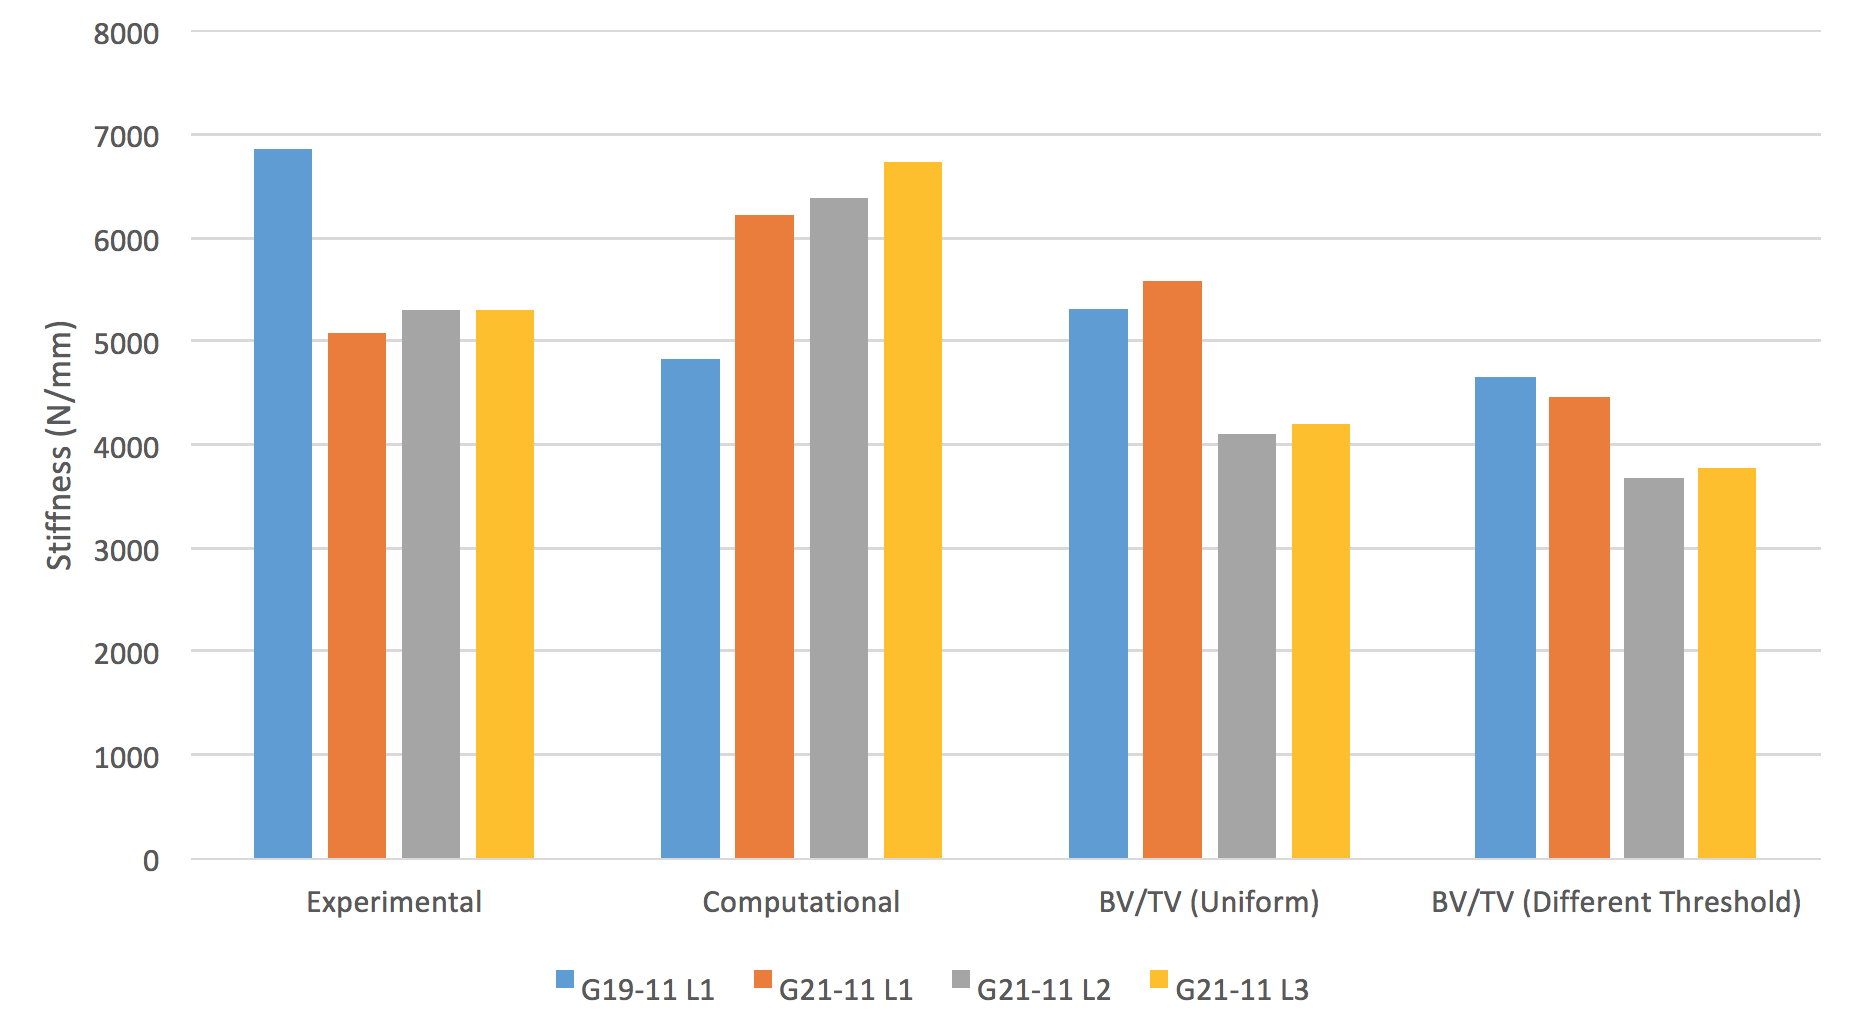
\includegraphics[width=6in]{Chapters/Chapter_HT_images/diffModellingMethods.png}
  \caption{The stiffness results of three different FE methods for four intact
    human vertebrae compared to the experimental stiffness results. Interest
    should be drawn to the ratio between specimen models rather than the values
    themselves, given that the conversion factors between greyscale values and
    Young's modulus have not been optimised at this stage. Results show the
    difference between the currently used method of modelling the vertebrae and
    the BV/TV based methods (both with uniform thresholds and different
    thresholds for each specimen).}
  \label{fig:diffModellingMethods}
\end{figure}




\subsubsection{Predicting Vertebral Yield Point}\label{predYield}

\subsubsection{Load Position Sensitivity}

\subsubsection{End-cap Depth \& Contact sensitivity}

\subsubsection{Modelling Augmentation}

Artificial brightening of regions surrounding
the internal cement, specifically concentrated areas of barium sulphate and the
artefacts this can cause affect the material properties that are applied to the
material.
To bypass this effect the two models, intact and post-augmentation models can be
registered - translating them into the same spacial location.
This allows the cement to be defined, masked and modelled based on the
post-augmentation scan and the remaining vertebra to be defined from the intact
scan, the same background used for the intact models.
While the shape of the vertebra may have been changed over the course of its
two loads, this change is less than what can be seen at 1 mm resolution.
Additionally regions that have experienced damage through the insertion of the
needle, yet do not contain cement will also be neglected using this method.
However, the same justification can be made, where this is unlikely to have any
affect at 1 mm resolution.


\section{Results}

\section{Discussion}

\section{Conclusion}







